\chapter{Proposed Methodology and System Design}
\label{chap:methodology}

\section{Overall System Architecture}
\label{sec:arch_overview}

The application follows a layered architecture in which each layer has a single, well-defined responsibility. Figure~\ref{fig:architecture} depicts the high-level data flow.

\begin{figure}[H]
\centering
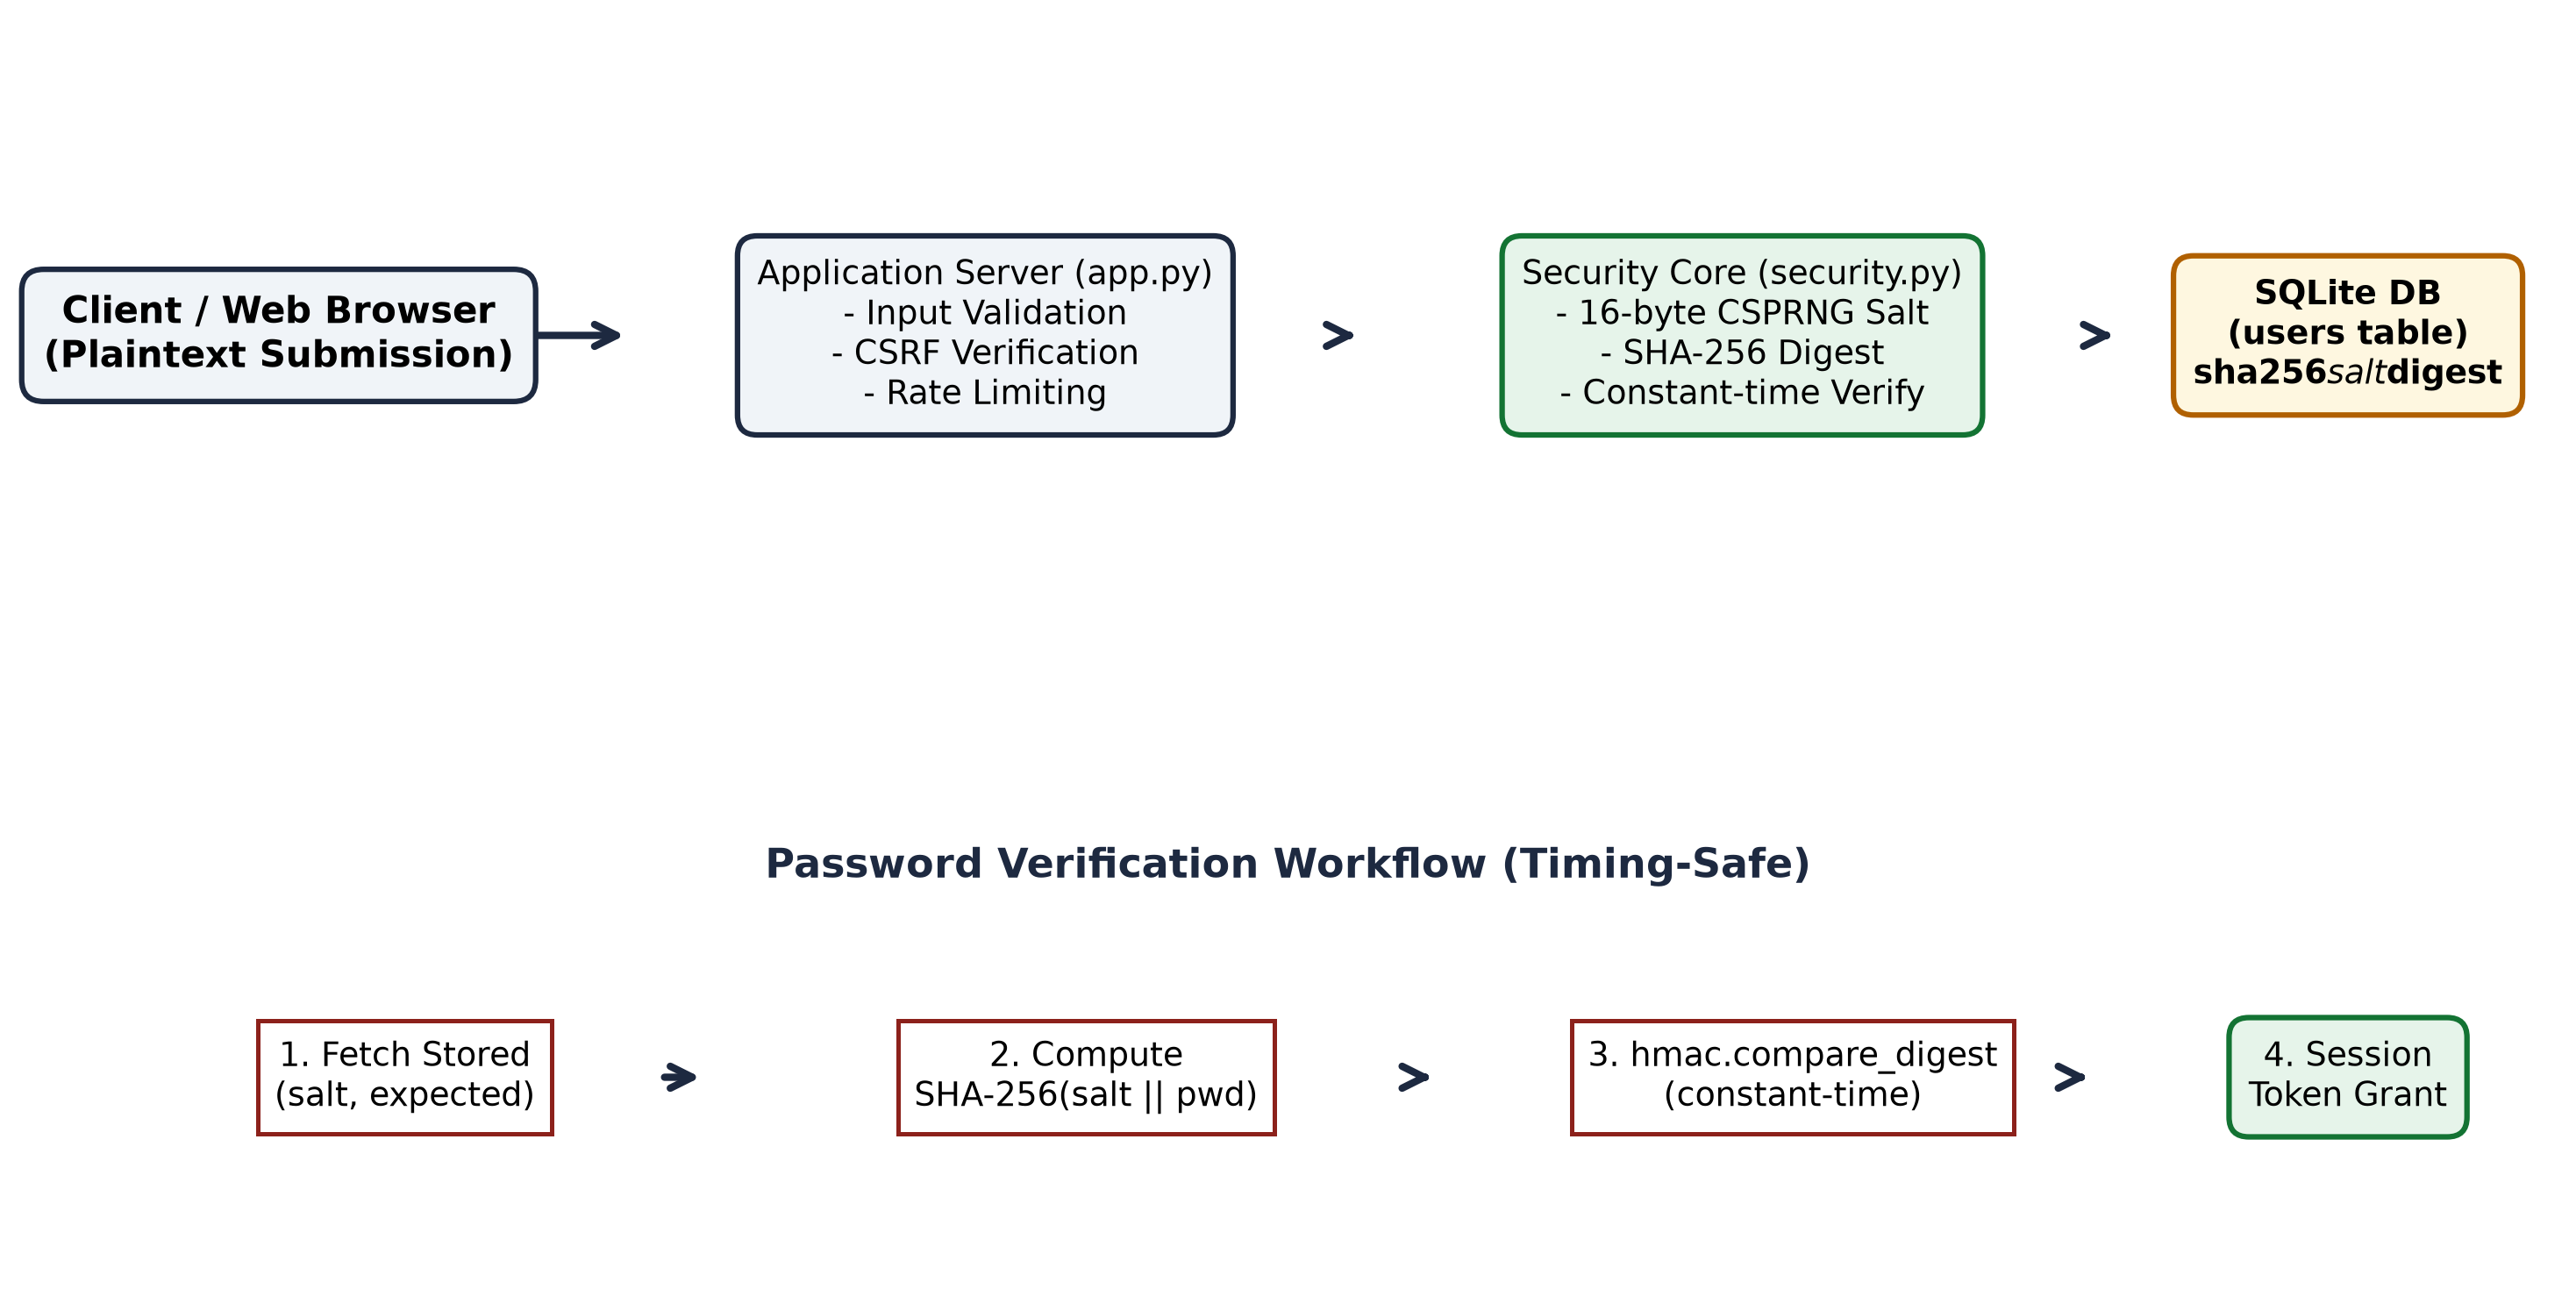
\includegraphics[width=0.95\textwidth]{architecture.png}
\caption{High-level system architecture showing layered data flow and verification workflow}
\label{fig:architecture}
\end{figure}

\begin{itemize}
  \item \textbf{Browser.} The client renders HTML pages served by the application and submits forms via HTTP POST. All cookies are \texttt{HttpOnly} and \texttt{SameSite=Lax} to mitigate XSS-based cookie theft and CSRF.

  \item \textbf{HTTP Handler (\texttt{app.py}).} A subclass of Python's \texttt{http.server.BaseHTTPRequestHandler} routes incoming requests, parses form data and cookies, enforces CSRF tokens, invokes rate limiting, delegates to the crypto layer for hash computation, and writes HTML responses.

  \item \textbf{Crypto Layer (\texttt{security.py}).} Contains all cryptographic operations: salt generation, SHA-256 hashing, constant-time comparison, session token generation, and CSRF token generation/validation using HMAC-SHA256.

  \item \textbf{Database Layer (\texttt{database.py}).} Wraps SQLite operations. All SQL statements use parameterised queries to eliminate SQL-injection risk. The layer exposes typed Python functions (not raw SQL) to the HTTP handler.

  \item \textbf{SQLite.} Stores the four tables described in Section~\ref{sec:arch_schema}. Never stores a password, session token, or any other secret in recoverable form.
\end{itemize}

\section{Cryptographic Module Design}
\label{sec:arch_crypto}

\subsection{The \texttt{hash\_password} Function}
\label{sec:arch_hash}

The primary credential-generation function accepts a plaintext password string and returns a self-describing encoded string containing the algorithm identifier, the hexadecimal salt, and the hexadecimal digest. The design steps are:

\begin{enumerate}
  \item \textbf{Salt generation.} Sixteen bytes are drawn from the OS CSPRNG via \texttt{secrets.token\_bytes(16)}, providing 128 bits of entropy. This salt is unique per registration event (or per password-change event).

  \item \textbf{Input construction.} The salt bytes are concatenated with the UTF-8 encoding of the password: $\text{data} = s \| \mathrm{encode}(p)$. This ensures that the hash function receives the full salted input as a single byte string, avoiding any ambiguity from separate HMAC-style key and data arguments.

  \item \textbf{Hash computation.} Python's \texttt{hashlib.sha256(data).digest()} computes the 32-byte SHA-256 digest in one call.

  \item \textbf{Encoding.} The encoded credential is assembled as: \newline
    \texttt{"sha256\$" + salt.hex() + "\$" + digest.hex()} \newline
    This yields a 32-character salt field and a 64-character digest field, separated by \texttt{\$} delimiters and prefixed by the algorithm name, for a total string length of approximately 103 characters.
\end{enumerate}

Algorithm~\ref{alg:hash_password} presents this logic in pseudocode.

\begin{algorithm}[H]
\caption{hash\_password($p$)}
\label{alg:hash_password}
\KwInput{Password string $p$}
\KwOutput{Encoded credential string}
$s \leftarrow \mathrm{CSPRNG}(16)$ \tcp*{16 random bytes}
$\text{data} \leftarrow s \;\|\; p.\mathrm{encode}(\texttt{utf-8})$\;
$d \leftarrow \mathrm{SHA\text{-}256}(\text{data})$\;
\Return $\texttt{"sha256\$"} \| \mathrm{hex}(s) \| \texttt{"\$"} \| \mathrm{hex}(d)$\;
\end{algorithm}

\subsection{The \texttt{verify\_password} Function}
\label{sec:arch_verify}

Password verification reconstructs the salted hash from the stored encoded string and compares it with the hash of the candidate password. Algorithm~\ref{alg:verify_password} details the procedure.

\begin{algorithm}[H]
\caption{verify\_password($p$, encoded)}
\label{alg:verify_password}
\KwInput{Candidate password $p$; encoded credential string}
\KwOutput{Boolean (True if password matches)}
Parse $\text{encoded}$ into $(\text{alg}, s_{\text{hex}}, d_{\text{hex}})$ by splitting on \texttt{"\$"}\;
\If{$\text{alg} \neq \texttt{"sha256"}$ \textbf{or} $|\text{parts}| \neq 3$}{
    \Return \textbf{False}\;
}
$s \leftarrow \mathrm{bytes.fromhex}(s_{\text{hex}})$\;
$d_{\text{expected}} \leftarrow \mathrm{bytes.fromhex}(d_{\text{hex}})$\;
$\text{data} \leftarrow s \;\|\; p.\mathrm{encode}(\texttt{utf-8})$\;
$d_{\text{actual}} \leftarrow \mathrm{SHA\text{-}256}(\text{data})$\;
\Return $\mathrm{hmac.compare\_digest}(d_{\text{actual}},\; d_{\text{expected}})$\;
\end{algorithm}

The use of \texttt{hmac.compare\_digest} in the final step is essential: it guarantees that the comparison time is independent of the content of the digests, eliminating timing side-channels as described in Section~\ref{sec:theory_timing}.

\subsection{Session Token Hashing}
\label{sec:arch_session_tokens}

Session tokens are 32-byte values produced by \texttt{secrets.token\_bytes(32)}. Before insertion into the \texttt{sessions} table, each token is hashed:

\begin{equation}
  t_{\text{stored}} = \mathrm{SHA\text{-}256}(t_{\text{raw}})
  \label{eq:session_token_hash}
\end{equation}

The raw token is placed in the client's \texttt{session\_id} cookie. During request handling, the handler hashes the incoming cookie value and queries the \texttt{sessions} table for a matching \texttt{token\_hash}. This ensures that compromise of the database does not yield usable session identifiers.

\subsection{CSRF Token Generation and Validation}
\label{sec:arch_csrf}

CSRF tokens are generated on login and stored in both the session record and an \texttt{HttpOnly} cookie. They are produced as:

\begin{equation}
  \tau = \mathrm{HMAC\text{-}SHA256}(t_{\text{raw}},\; \texttt{"csrf"}).\mathrm{hex}()
  \label{eq:csrf_generation}
\end{equation}

Every state-changing POST handler reads the CSRF token from the submitted form field and from the server-side session record, then compares them using \texttt{hmac.compare\_digest}. A mismatch returns HTTP~403 without performing any further processing.

\section{Database Schema}
\label{sec:arch_schema}

The SQLite database contains four tables. All tables use the \texttt{STRICT} keyword where supported to enforce column types.

\begin{table}[H]
\centering
\caption{Database schema: \texttt{users} table}
\label{tab:schema_users}
\begin{tabularx}{\textwidth}{|l|l|X|}
\hline
\textbf{Column} & \textbf{Type} & \textbf{Description} \\\hline
\texttt{id}              & INTEGER PRIMARY KEY & Auto-increment identifier \\\hline
\texttt{username}        & TEXT UNIQUE NOT NULL & Normalised lowercase username \\\hline
\texttt{password\_hash}  & TEXT NOT NULL & Encoded credential: \texttt{sha256\$<salt\_hex>\$<hash\_hex>} \\\hline
\texttt{created\_at}     & TEXT NOT NULL & ISO-8601 timestamp of registration \\\hline
\texttt{last\_login}     & TEXT & ISO-8601 timestamp of most recent successful login \\\hline
\end{tabularx}
\end{table}

\begin{table}[H]
\centering
\caption{Database schema: \texttt{sessions} table}
\label{tab:schema_sessions}
\begin{tabularx}{\textwidth}{|l|l|X|}
\hline
\textbf{Column} & \textbf{Type} & \textbf{Description} \\\hline
\texttt{id}            & INTEGER PRIMARY KEY & Auto-increment identifier \\\hline
\texttt{user\_id}      & INTEGER REFERENCES users & Foreign key to \texttt{users.id} \\\hline
\texttt{token\_hash}   & TEXT UNIQUE NOT NULL & SHA-256 of raw session token \\\hline
\texttt{csrf\_token}   & TEXT NOT NULL & HMAC-SHA256 CSRF token bound to session \\\hline
\texttt{expires\_at}   & TEXT NOT NULL & ISO-8601 expiry timestamp \\\hline
\texttt{created\_at}   & TEXT NOT NULL & ISO-8601 creation timestamp \\\hline
\end{tabularx}
\end{table}

\noindent The \texttt{attempts} table records failed login attempts (username, timestamp, IP address) to support rate limiting. The \texttt{activity} table records successful login and logout events for audit purposes.

\section{Rate Limiting Design}
\label{sec:arch_rate_limiting}

The rate limiter uses a bucket-based algorithm with a 5-minute rolling window. On each authentication attempt, the system:

\begin{enumerate}
  \item Queries the \texttt{attempts} table for all failed attempts by the given username in the past 300 seconds.
  \item If the count is $\geq 5$, the request is rejected with an HTTP 429 response before any hash computation is performed.
  \item If the authentication succeeds, all attempt records for that username are deleted (clearing the bucket).
  \item If the authentication fails, a new record is inserted into \texttt{attempts}.
\end{enumerate}

Importantly, the rate limiter runs \emph{before} the hash computation on failure paths, so it does not introduce a timing signal about the validity of the username. A ``dummy'' \texttt{verify\_password} call (computing \texttt{hash\_password("dummy")} and immediately discarding the result) is executed even when no matching user is found, ensuring that the response time for invalid usernames matches the response time for valid usernames with incorrect passwords.
